%\section{Une section}

% remarque : pour qu'un mot se retrouve dans le lexique : \MotDefinition{asymptote horizontale}{} 

\begin{aconnaitre}
Lorsqu'on représente un solide en \MotDefinition{perspective cavalière}{} :
\begin{itemize}
 \item La face avant est représentée en vraie grandeur ;
 \item Les arêtes parallèles sont représentées par des segments parallèles ;
 \item Les arêtes cachées sont dessinées en pointillés.
 \end{itemize}
\end{aconnaitre}

\begin{methode*1}[Représenter en perspective cavalière]

 \begin{exemple*1}
 
 \begin{minipage}[c]{0.62\linewidth}
 Complète la représentation en perspective cavalière du pavé droit ci‑contre.
  \end{minipage} \hfill%
  \begin{minipage}[c]{0.32\linewidth} 
   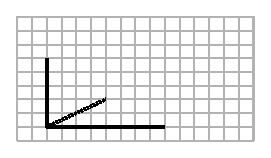
\includegraphics[width=3.3cm]{persp_xyz}
   \end{minipage} \\[1.4em]
   
 \begin{minipage}[t]{0.3\linewidth}   
On commence par la face avant, en vraie grandeur.
  \end{minipage} \hfill%
  \begin{minipage}[t]{0.3\linewidth}
On trace les arêtes transversales, parallèles et de même longueur, mais pas en vraie grandeur.
  \end{minipage} \hfill%
   \begin{minipage}[t]{0.3\linewidth}   
On finit par la face arrière, en vraie grandeur.
   \end{minipage} \\
   
 \begin{minipage}[c]{0.3\linewidth}     
\begin{center} 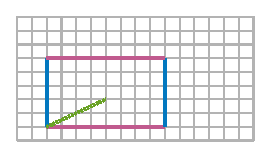
\includegraphics[width=3.3cm]{persp_rectangle1} \end{center}
  \end{minipage} \hfill%
  \begin{minipage}[c]{0.3\linewidth}
\begin{center} 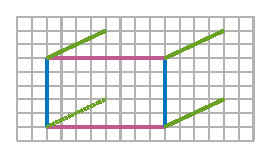
\includegraphics[width=3.3cm]{persp_rectangle2} \end{center}
  \end{minipage} \hfill%
   \begin{minipage}[c]{0.3\linewidth}   
\begin{center} 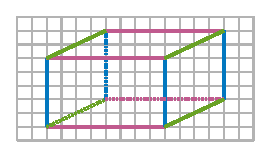
\includegraphics[width=3.3cm]{persp_rectangle3} \end{center}
   \end{minipage} \\
 \end{exemple*1}

 \begin{exemple*1}
Trace un prisme droit à base triangulaire en perspective cavalière. \\[1em]
 \begin{minipage}[c]{0.30\linewidth}
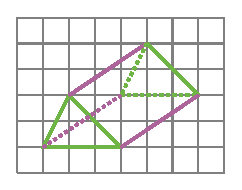
\includegraphics[width=3cm]{persp_triangle} 
  \end{minipage} \hfill%
  \begin{minipage}[c]{0.76\linewidth} 
Les \textcolor{H1}{\textbf{bases}} de ce prisme droit sont des triangles parallèles et superposables. On les représente en vraie grandeur. \\[0.5em]
Les \textcolor{C1}{\textbf{arêtes latérales}} de ce prisme sont parallèles et de même longueur. On les représente par des segments parallèles de même longueur. \\[0.5em]
On trace en pointillés les arêtes cachées. 
   \end{minipage} \\
 \end{exemple*1}

 \exercice  
Complète les représentations en perspective cavalière des deux pavés ci‑dessous :
\begin{colenumerate}{2}
 \item 
 
 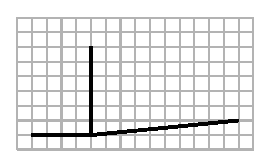
\includegraphics[width=4.2cm]{persp_ex1} 
 \item 
 
 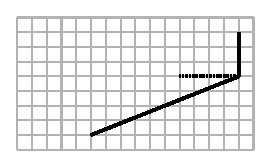
\includegraphics[width=4.2cm]{persp_ex2} 
 \end{colenumerate}
%\correction

 \exercice
 
 \begin{minipage}[c]{0.48\linewidth}
Reproduis puis complète le tracé en perspective cavalière du prisme droit ci-contre :
  \end{minipage} \hfill%
  \begin{minipage}[c]{0.48\linewidth} 
\begin{center} 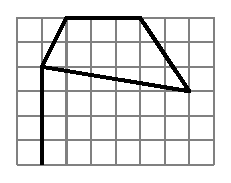
\includegraphics[width=3cm]{persp_ex3} \end{center}
  \end{minipage} \\
%\correction

 \end{methode*1}
 
 %%%%%%%%%%%%%%%%%%%%%%%%%%%%%%%%%%%%%%%%%%%%%%%%%%%%%%%%%%%%%%%%%%%%%%%%

\begin{methode*1}[Construire un patron]

 \begin{exemple*1}
Construis un patron d'un pavé droit $ABCDEFGH$ tel que $AB = 3$ cm, $AD = 4$ cm et $AE = 5$ cm. \\[1.2em]
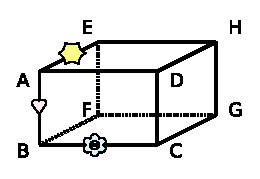
\includegraphics[width=4.1cm]{patron1} 

 \begin{minipage}[c]{0.6\linewidth}
Un pavé droit comprend trois paires de faces rectangulaires parallèles et de mêmes dimensions.
\begin{itemize}
 \item Les faces ${\textcolor{J1}{ABCD}}$ et $\textcolor{J1}{EFGH}$ mesurent 3 cm par 4 cm ; 
 \item Les faces $\textcolor{C2}{AEHD}$ et $\textcolor{C2}{BFGC}$ mesurent 4 cm par 5 cm ; 
 \item Les faces $\textcolor{H1}{ABFE}$ et $\textcolor{H1}{DCGH}$ mesurent 3 cm par 5 cm.
 \end{itemize}
  \end{minipage} \hfill%
  \begin{minipage}[c]{0.38\linewidth} 
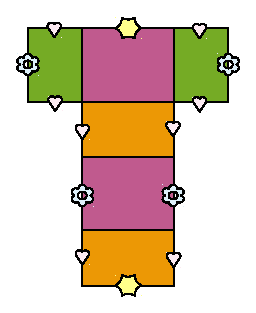
\includegraphics[width=4.1cm]{patron2}  
  \end{minipage} \\  
   
Pour obtenir le patron, on peut les disposer « en $T$ ». 
 \end{exemple*1}

 \begin{exemple*1}
Dessine le patron d'un prisme droit dont la base est un triangle de côtés 5 cm, 4 cm et 3 cm, et dont la hauteur est 2 cm. \\[1em]
   
 \begin{minipage}[c]{0.3\linewidth}     
\vspace{-0.2cm}
\begin{center} 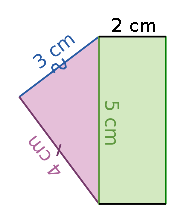
\includegraphics[width=2.2cm]{patron3} \end{center}
  \end{minipage} \hfill%
  \begin{minipage}[c]{0.3\linewidth}
\begin{center} 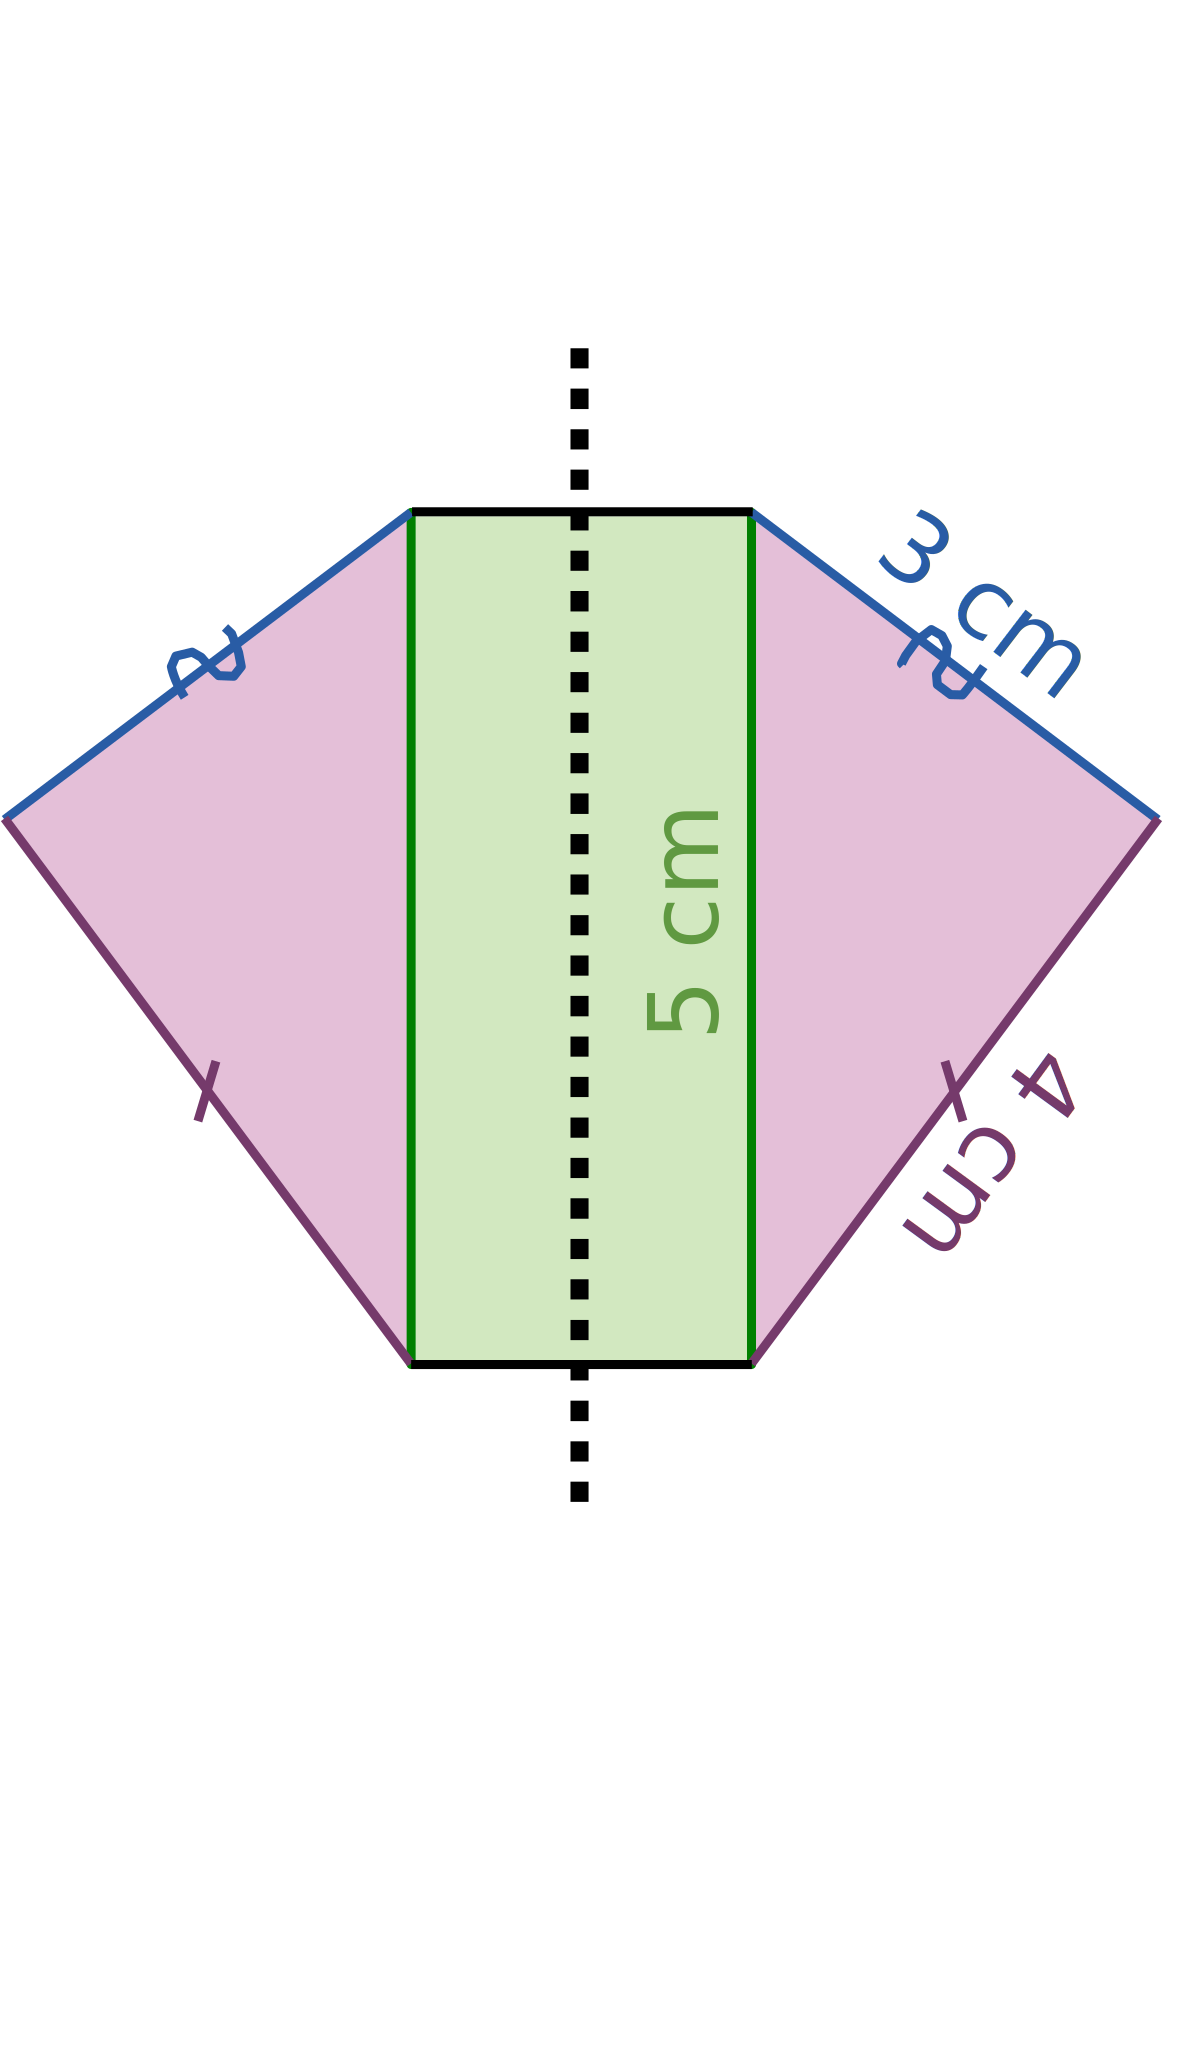
\includegraphics[width=3.4cm]{patron4} \end{center}
  \end{minipage} \hfill%
   \begin{minipage}[c]{0.3\linewidth}   
\begin{center} 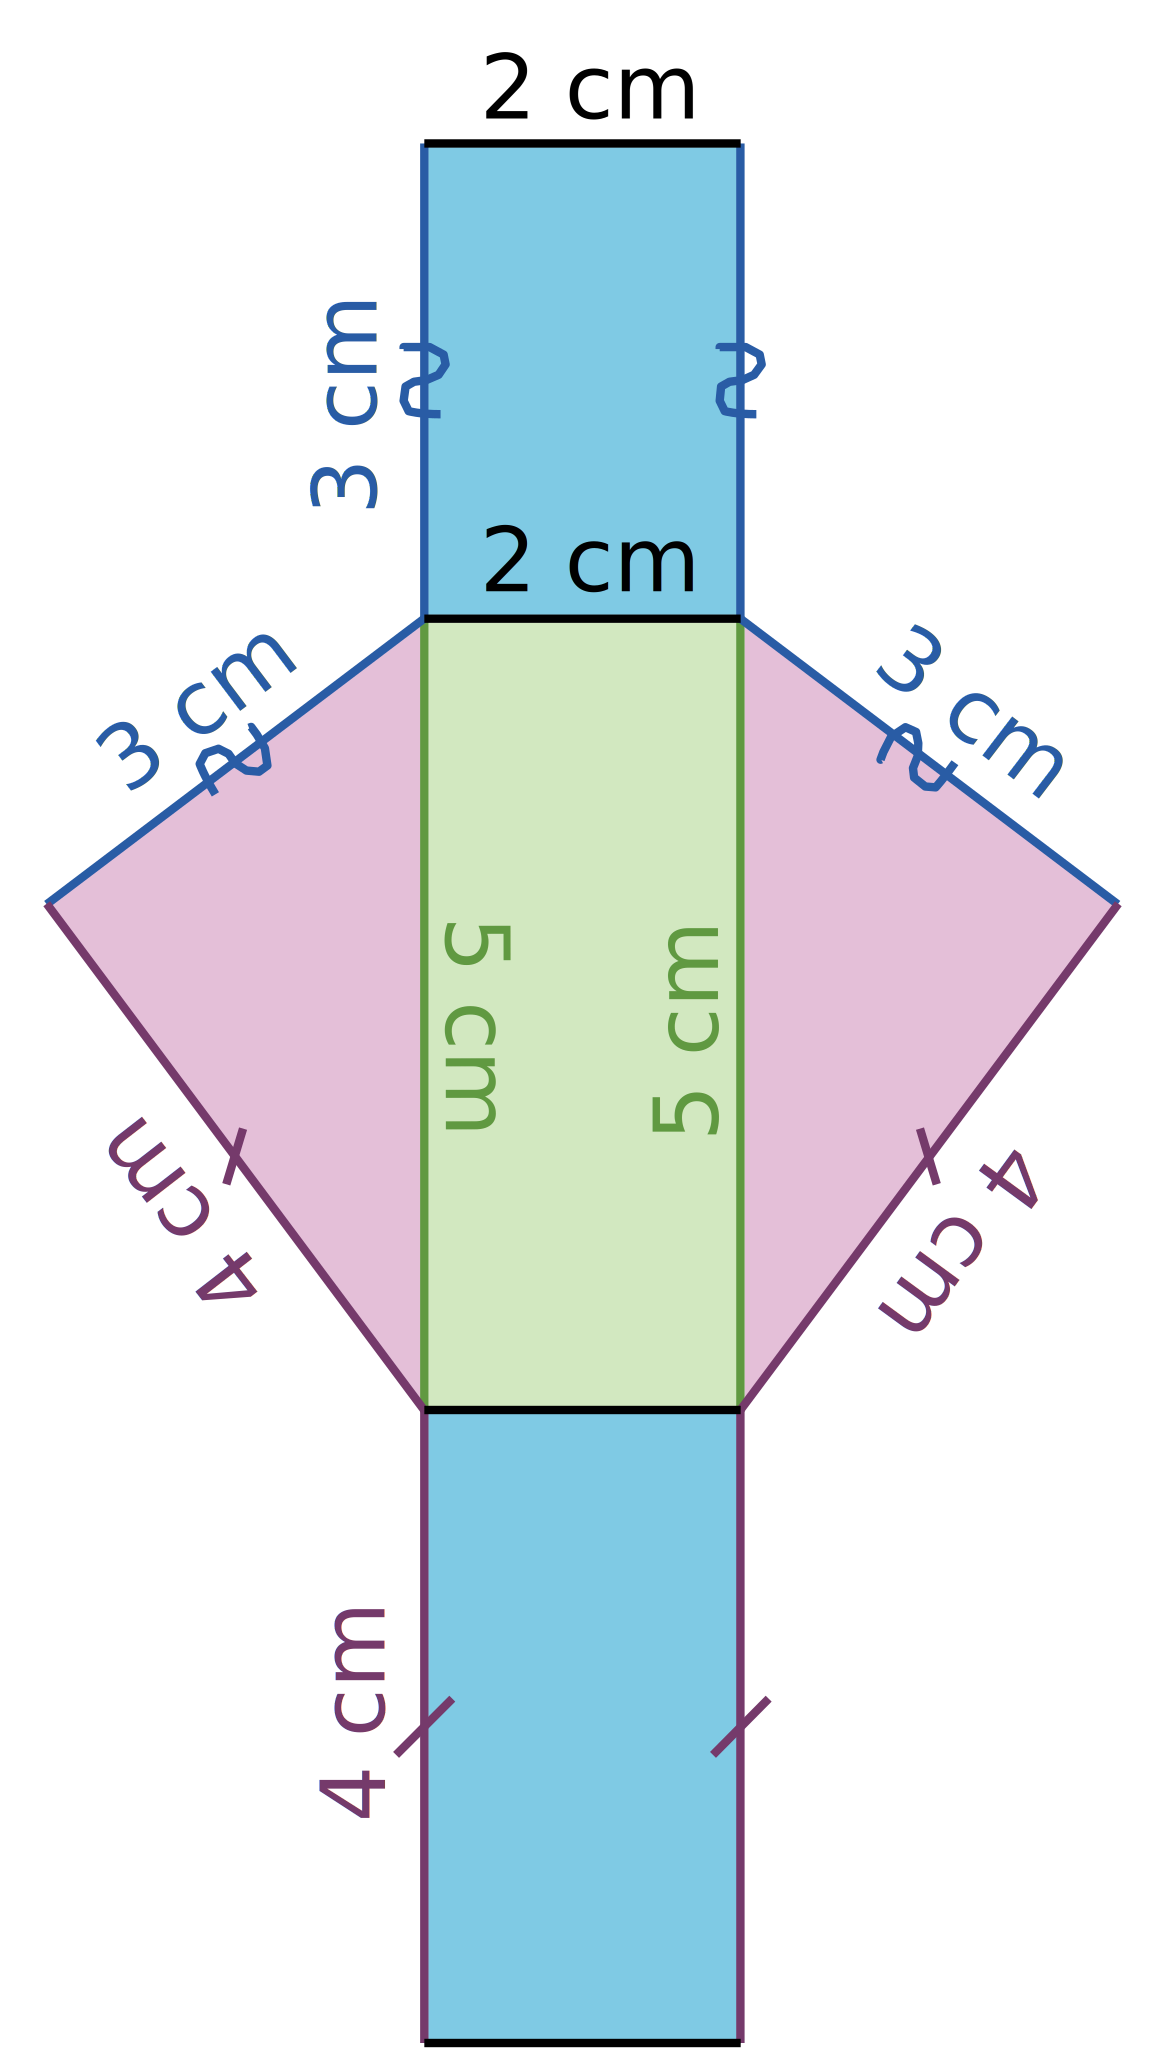
\includegraphics[width=3.6cm]{patron5} \end{center}
   \end{minipage} \\
   
 \begin{minipage}[t]{0.3\linewidth}      
On construit une des \textcolor{C2}{\textbf{bases}}, qui est un triangle, puis on trace une \textcolor{H2}{\textbf{face latérale}} qui est un rectangle dont les côtés sont un côté de la base et la hauteur du prisme droit.
  \end{minipage} \hfill%
  \begin{minipage}[t]{0.3\linewidth}
On trace la seconde \textcolor{C2}{\textbf{base}}, qui est un triangle symétrique au premier par rapport à l'un des axes de symétrie du rectangle.
  \end{minipage} \hfill%
   \begin{minipage}[t]{0.3\linewidth}   
On complète le patron en traçant les deux dernières \textcolor{U1}{\textbf{faces latérales}} du prisme droit, qui sont des rectangles.
   \end{minipage} \\
 \end{exemple*1}

 \exercice  
Construis un patron d'un pavé droit de dimensions 4,5 cm ; 6,2 cm et 3 cm.
%\correction

 \exercice  
Construis un patron d'un cube de côté 6,5 cm.
%\correction

 \exercice  
Dessine un patron d'un prisme droit de hauteur 3 cm ayant pour base un triangle $ABC$ rectangle en $A$ tel que $AB = 2,5$ cm et $AC = 4$ cm.
%\correction

 \end{methode*1}
 
 %%%%%%%%%%%%%%%%%%%%%%%%%%%%%%%%%%%%%%%%%%%%%%%%%%%%%%%%%%%%%%%%%%%%%%%%
 
 \begin{aconnaitre}
   \begin{minipage}[t]{0.48\linewidth}
  \begin{center} 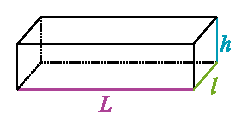
\includegraphics[width=3.8cm]{vol_parall} \end{center}
  \end{minipage} \hfill%
   \begin{minipage}[t]{0.48\linewidth}    
  \begin{center}  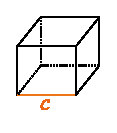
\includegraphics[width=1.5cm]{vol_cube} \end{center}
   \end{minipage} \\
   \begin{minipage}[t]{0.48\linewidth}
  \begin{center} Volume du parallélépipède rectangle \end{center}
  \begin{center} $V = \textcolor{C1}{L} \cdot \textcolor{H1}{l} \cdot \textcolor{U1}{h}$ \end{center}
  \end{minipage} \hfill%
   \begin{minipage}[t]{0.48\linewidth}  
  \begin{center} Volume du cube \end{center}
  \begin{center} $V = \textcolor{J1}{c} \cdot \textcolor{J1}{c} \cdot  \textcolor{J1}{c}$ \end{center}
   \end{minipage} \\[1em]
Les longueurs doivent être exprimées dans la même unité.
\end{aconnaitre}

\begin{methode*1}[Calculer le volume d'un cube et d'un parallélépipède rectangle]

 \begin{remarque}
Un parallélépipède rectangle peut également s'appeler un \textbf{pavé droit}.
 \end{remarque}
 
 \begin{exemple*1}
Calcule le volume d'un pavé droit de 32 mm de longueur, 2,5 cm de largeur et 0,4 dm de hauteur. \\[1em]
\begin{tabular}{lll} 
 $V = \textcolor{C1}{L} \cdot \textcolor{H1}{l} \cdot \textcolor{U1}{h}$ & $\longrightarrow$ & On écrit la formule. \\
 $V = \textcolor{C1}{3,2}\,\text{cm} \cdot \textcolor{H1}{2,5}\,\text{cm} \cdot \textcolor{U1}{4}\,\text{cm}$ ; & $\longrightarrow$ & On remplace par les données \\
 $V = 32\,\text{cm}$\up{3} & & numériques exprimées dans la  \\
 & & même unité : \\
 & & $32\,\text{mm} = 3,2\,\text{cm}$ et $0,4\,\text{dm} = 4\,\text{cm}$. \\
 \end{tabular}
 Le volume du pavé droit est de 32 cm\up{3}.
 \end{exemple*1}


 \exercice  
Calcule le volume d'un cube de 6,1 dm de côté.
%\correction

 \exercice  
\begin{minipage}[c]{0.48\linewidth}
Calcule le volume du solide ci‑contre :
 \end{minipage} \hfill%
 \begin{minipage}[c]{0.28\linewidth}
  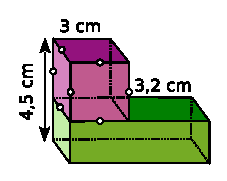
\includegraphics[width=3.4cm]{solide_rosevert}
  \end{minipage} \\
%\correction

 \end{methode*1}
 
 %%%%%%%%%%%%%%%%%%%%%%%%%%%%%%%%%%%%%%%%%%%%%%%%%%%%%%%%%%%%%%%%%%%%%%%%